\lecture{16}{18 May 2023 }{Inner Product and Normed Spaces}

\subsection{Motivating Examples on Inner Produc and Norm}
\begin{remark}
    For the scope of this lecture, we shall restrict our field \(\bbk\) to either \(\bbr\) or \(\bbc\) (I'll denote \(\bbr / \bbc\)), which are called ``normed'' fields, that are roughly fields in which we can make sense of the notion of distance.
\end{remark}

\begin{example}
    On \(\bbr, \alpha \in \bbr \leadsto \abs{\alpha}\)

    On \(\bbc, \beta = a + bi \in \bbc \leadsto \abs{\beta} = \abs{\beta \cdot \conj{\beta}}^{\frac{1}{2}} = \sqrt{a^2 + b^2}\)
\end{example}

Let \(V\) be a vector space over \(\bbr /\bbc\), then we now want to talk about ``distancne'' in \(V\)

\begin{example}
    If \(V = \bbr^d\). Let \begin{align*}
        x & = (x_1, x_2, \dots, x_d) \in \bbr^d \\
        y & = (y_1, y_2, \dots, y_d) \in \bbr^d
    \end{align*}

    Then the ``dot product'' is defined over \(\bbr^d\) as follows: \[
        \innerproduct{x}{y} = x \cdot y^T = \sum x_i y_i \in \bbr
    \]
    Then \(\innerproduct{x}{x} = \sum x_i^2\) and \(\norm{x} \coloneqq \sqrt{\innerproduct{x}{x}}\) is the distance to origin.
\end{example}


\begin{example}
    If \(V = \bbc^d\). Let \begin{align*}
        x & = (x_1, x_2, \dots, x_d) \in \bbc^d \\
        y & = (y_1, y_2, \dots, y_d) \in \bbc^d
    \end{align*}

    Then the ``dot product'' is defined over \(\bbc^d\) as follows: \[
        \innerproduct{x}{y} = x \cdot \conj{y} =\sum x_i \conj{y_i}  \in \bbc
    \]
    Then \(\norm{x} \coloneqq \sqrt{\innerproduct{x}{x}} = \sqrt{x \conj{x}}\), which obviously also applies to \(\bbr\).

    If \(x = (x_1, x_2) \in \bbc^2\) then \(\norm{x} = \sqrt{x_1 \conj{x_1} + x_2 \conj{x_2}} = \sqrt{\abs{x_1}^2 + \abs{x_2}^2}\)
\end{example}

\subsection{Inner Product Space}
\begin{definition} {Inner Product Space}
    An \textbf{inner product space} is a vector space \(V\) over \(\bbr / \bbc\), together with an ``inner product mapping'': \[
        \innerproduct{}{}: V \times V \to \bbk (= \bbr / \bbc) \st
    \]
    \begin{enumerate}
        \item \(\innerproduct{x}{y} = \conj{\innerproduct{y}{x}}\) (over \(\bbr\), this is simply an equality without the conjugate)
        \item \(\innerproduct{\alpha x + \beta y}{z} = \alpha \innerproduct{x}{z} + \beta \innerproduct{y}{z}\)
        \item \(\innerproduct{x}{x} \leq 0 \forall x \in V\) and \[
                  \innerproduct{x}{x} = 0 \Leftrightarrow x = 0
              \]

              This non-negative requirement strengthens our understanding of this as a notion of ``distance''!
    \end{enumerate}
\end{definition}

If \((V, \innerproduct{}{})\) is an inner product space as such, we can write \[
    \norm{x} \coloneqq \sqrt{\innerproduct{x}{x}}
\]
\begin{observe}
    \(\innerproduct{x}{y}\) is linear with respect to the first component, and is ``conjugate linear'' with respect to the second component. While the first part is clue from property (2), the second part can be shown as follows:
    \begin{align*}
        \innerproduct{x}{\beta_y + z} & = \conj{\beta\innerproduct{y}{x} + \innerproduct{z}{x}}                \\
                                      & = \conj{\beta} \conj{\innerproduct{y}{x}} + \conj{\innerproduct{z}{x}} \\
                                      & = \conj{\beta} \innerproduct{x}{y} + \innerproduct{x}{z}
    \end{align*}
\end{observe}
\begin{lemma} [Cauchy-Schwarz]
    Let \((V, \innerproduct{}{})\) be an inner product space. Then \(\forall x, y \in V  \), \[
        \abs{\innerproduct{x}{y}} \leq \norm{x} \norm{y}
    \]
\end{lemma}

\begin{proof} {Lemma}
    We shall prove it for the case \(\bbk = \bbr\); when \(\bbk = \bbc\) the proof is very similar.

    Observe than if \(y= 0 \implies \innerproduct{x}{y} = 0, \norm{y} = 0\), this case is trivial.

    Therefore let's assume that \(y \neq 0\).

    Consider \begin{align*}
        0 & \leq \innerproduct{x - ty}{x - ty} \:\text{for some}\:  t \in \bbr                                                      \\
          & = \innerproduct{x}{x - ty} - \innerproduct{ty}{ x- ty}                                                                  \\
          & = \innerproduct{x}{x} - \innerproduct{x}{ty} - \innerproduct{ty}{x} + \innerproduct{ty}{ty}                             \\
          & = \norm{x}^2 - 2t \innerproduct{x}{y} + t^2 \norm{y}^2 (\innerproduct{x}{y} = \innerproduct{y}{x} \:\text{over}\: \bbr) \\
    \end{align*}

    Therefore, \[
        \norm{x}^2 + t^2 \norm{y}^2 \geq 2t \innerproduct{x}{y}
    \]

    In particular, we can choose a convenient value for \(t = \frac{\innerproduct{x}{y}}{\norm{y}^2} \), then: \begin{align*}
        \norm{x}^2 + \dfrac{\abs{\innerproduct{x}{y}}^2 }{\norm{y}^2} & \geq \dfrac{2\abs{\innerproduct{x}{y}}^2 }{\norm{y}^2} \\
        \implies \norm{x}^2 \norm{y}^2                                & \geq \abs{\innerproduct{x}{y}}^2                       \\
        \implies \norm{x} \norm{y}                                    & \geq \abs{\innerproduct{x}{y}}
    \end{align*}
\end{proof}

\begin{corollary} [Triangle Inequality]
    If \(x, y \in V\) where \((V, \innerproduct{}{})\) is an inner product space over \(\bbr / \bbc\) then \[
        \norm{x + y} \leq \norm{x} + \norm{y}
    \]

    Also, \[
        \norm{x - y} \leq \norm{x} + \norm{y}
    \]
\end{corollary}

\begin{proof} {Corollary}
    WTS: \[
        \norm{x + y} \leq \norm{x} + \norm{y} \Leftrightarrow \innerproduct{x+y}{x+y} \leq \norm{x}^2 + \norm{y}^2 + 2 \norm{x}\norm{y}
    \]
    The equivalence is possible since both sides are non-negative. Expanding:
    \[
        LHS = \norm{x}^2 + \norm{y}^2 + \innerproduct{x}{y} + \innerproduct{y}{x}
    \]
    We know from Cauchy-Schwarz that \(\norm{x} \norm{y} \geq \abs{\innerproduct{x}{y}}\), and therefore WTS that \[
        \innerproduct{x}{y} + \innerproduct{y}{x} \leq 2 \abs{\innerproduct{x}{y}}
    \]

    But this is borderline obvious, let \(\innerproduct{x}{y} = m = a + bi\) then : \[
        m + \conj{m} = 2 a \leq 2 \sqrt{a^2 + b^2} = 2 \abs{\innerproduct{x}{y}}
    \]
\end{proof}

This exploration of the relationship between the norm and inner product gives us a more abstract idea of the norm!

\subsection{Normed Space}
\begin{definition} {Normed Space}
    A \textbf{normed} vector space is a vector space \(V\) over \(\bbk = \bbr / \bbc\), equipped with a function: \[
        \norm{\cdot}: V \to \bbr \st
    \]
    \begin{enumerate}
        \item \(\norm{x} \leq 0, \norm{x} = 0 \Leftrightarrow x = 0 \)
        \item \(\forall \alpha \in \bbk, \norm{\alpha x} = \abs{\alpha} \norm{x}\)
        \item \(\norm{x + y} \leq \norm{x} + \norm{y} \forall x, y \in V\)
    \end{enumerate}
\end{definition}

\begin{remark}
    It is clear from our exploration above, that if \((V, \innerproduct{}{})\) is an inner product space over \(\bbr / \bbc\) then we can build \((V, \norm{\cdot})\) to be a normed space, by defining \[
        \norm{x} \coloneqq \sqrt{\innerproduct{x}{x}}
    \]
\end{remark}

\begin{definition} {Perpendicular, Orthogonal}
    Let \((V, \innerproduct{}{})\) be an inner product space over \(\bbr / \bbc\). Then \(v, w \in V\) are said to be \textbf{perpendicular} to each other if \[
        \innerproduct{v}{w} = 0
    \]
    and we write \[
        v \perp w
    \]

    In general, if \(E, F \subseteq V\) are 2 subspaces, then \(E \perp F\) if \(x \perp y \forall x \in E, \forall y \in F\)

    Similarly, define \(x \perp E\) if \(x \in V, x \perp w \forall w \in E\)
\end{definition}

\begin{observe}
    If \(x \perp y\) then \begin{align*}
        \norm{x+y}^2 & =  \innerproduct{x+y}{x+y}                                                              \\
                     & = \innerproduct{x}{x} + \innerproduct{x}{y} + \innerproduct{y}{x} + \innerproduct{y}{y} \\
                     & = \norm{x}^2 + \norm{y}^2
    \end{align*}
    \textbf{Pythagoras!}
\end{observe}

\subsection{Orthogonal System of Vectors}
\begin{definition} {Orthogonal System of Vectors}
    Let \(\{v_1, v_2, \dots, v_r\}\) be vectors \(V\), then they are called an \textbf{orthogonal system of vectors} if \(v_i \perp v_j \forall i \neq j\)
\end{definition}

\begin{lemma}
    If \(\{v_i\}\) is an orthogonal system then \[
        \norm{\sum_{i=1}^{r} \alpha_i v_i}^2 = \sum_{i=1}^{r} \abs{\alpha_i}^2 \norm{v_i}^2
    \]
    where \(a_i \in \bbk\). The proof of which shall be left as an exercise.
\end{lemma}

\begin{corollary}
    If \(\{v_i\}, v_i \neq 0\) is an orthogonal system then they are linearly independent
\end{corollary}

\begin{proof} {Corollary}
    Suppose \(\sum \alpha_i v_i = 0 \implies \norm{\sum \alpha_i v_i}^2 = 0 \implies \sum \abs{\alpha_i}^2 \norm{v_i}^2 = 0 \implies \abs{\alpha_i} = 0 \implies \alpha_i = 0\)
\end{proof}

\begin{definition} {Orthonormal}
    \(\{v_1, v_2, \dots, v_r\}\) is \textbf{orthonormal} if it is orthogonal and \(\norm{v_i} = 1 \forall i\). It is easy to see that we can always transform an orthogonal system to an orthonormal system of vectors, simply by dividing each vector by their norm.
\end{definition}

\subsection{Orthogonal Projection}



\tikzset{every picture/.style={line width=0.75pt}} %set default line width to 0.75pt        

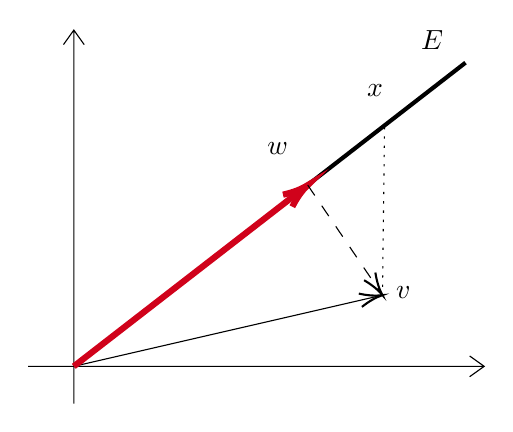
\begin{tikzpicture}[x=0.75pt,y=0.75pt,yscale=-1,xscale=1]
%uncomment if require: \path (0,226); %set diagram left start at 0, and has height of 226

%Shape: Axis 2D [id:dp40406254328760394] 
\draw  (220,187.3) -- (439.67,187.3)(241.97,25.3) -- (241.97,205.3) (432.67,182.3) -- (439.67,187.3) -- (432.67,192.3) (236.97,32.3) -- (241.97,25.3) -- (246.97,32.3)  ;
%Straight Lines [id:da08092535764639175] 
\draw [color={rgb, 255:red, 0; green, 0; blue, 0 }  ,draw opacity=1 ][line width=1.5]    (241.97,187.3) -- (430.67,41) ;
%Straight Lines [id:da6958476015789383] 
\draw    (241.97,187.3) -- (388.72,153.45) ;
\draw [shift={(390.67,153)}, rotate = 167.01] [color={rgb, 255:red, 0; green, 0; blue, 0 }  ][line width=0.75]    (10.93,-3.29) .. controls (6.95,-1.4) and (3.31,-0.3) .. (0,0) .. controls (3.31,0.3) and (6.95,1.4) .. (10.93,3.29)   ;
%Straight Lines [id:da41896114397568796] 
\draw [color={rgb, 255:red, 208; green, 2; blue, 27 }  ,draw opacity=1 ][line width=2.25]    (241.97,187.3) -- (339.08,112.08) -- (351.5,102.45) ;
\draw [shift={(354.67,100)}, rotate = 142.24] [color={rgb, 255:red, 208; green, 2; blue, 27 }  ,draw opacity=1 ][line width=2.25]    (12.24,-3.68) .. controls (7.79,-1.56) and (3.71,-0.33) .. (0,0) .. controls (3.71,0.33) and (7.79,1.56) .. (12.24,3.68)   ;
%Straight Lines [id:da6782950706670643] 
\draw  [dash pattern={on 4.5pt off 4.5pt}]  (354.67,100) -- (389.54,151.35) ;
\draw [shift={(390.67,153)}, rotate = 235.81] [color={rgb, 255:red, 0; green, 0; blue, 0 }  ][line width=0.75]    (10.93,-3.29) .. controls (6.95,-1.4) and (3.31,-0.3) .. (0,0) .. controls (3.31,0.3) and (6.95,1.4) .. (10.93,3.29)   ;
%Straight Lines [id:da754128340594165] 
\draw  [dash pattern={on 0.84pt off 2.51pt}]  (391.67,72) -- (390.67,153) ;

% Text Node
\draw (408,24.4) node [anchor=north west][inner sep=0.75pt]    {$E$};
% Text Node
\draw (334,78.4) node [anchor=north west][inner sep=0.75pt]    {$w$};
% Text Node
\draw (396,147.4) node [anchor=north west][inner sep=0.75pt]    {$v$};
% Text Node
\draw (382,50.4) node [anchor=north west][inner sep=0.75pt]    {$x$};


\end{tikzpicture}


We want to find \(w \in E \st (x - w) \perp w\)

\begin{definition} {Projection}
    Let \(V\) be an inner product space, \(E \subseteq V\) be a subspae. Define \[
        pr_E: V \to E
    \]
    to be a projection \st \(\forall x \in V, x - pr_E(x) \perp pr_E(x)\)

    So far, we do not know if it even exists, and if it does whether it's unique.
\end{definition}

\vspace{1cm}
\begin{lemma}
    Let \(v \in V, w \in E\). Suppose \(v - w \perp w\) then \(\forall x \in E, \norm{v - w} \leq \norm{v - x}\). Essentially, the projection gives the minimum distance from \(V \to E\), and it is unique.
\end{lemma}

\begin{proof} {Lemma}
    We first enforce a stronger definition for projection, that is \[
        x - pr_E(x) \perp E
    \]
    The proof for the general case is similar to this.

    We first prove that if there exists \(w = pr_E(x) \in E\), then it is unique.

    Write \(\delta \coloneqq w - x\) then \(v - x = (v - w) + (w - x) = (v- w) + \delta\)

    But \(\delta = w - x \in E\). Since \(v - w \perp E \implies v - w \perp \delta\). Then,
    \begin{align*}
        \norm{v-x}^2        & = \norm{(v-w) + \delta} ^2                                       \\
                            & = \norm{v-w}^2 + \norm{\delta}^2 (\Leftarrow (v-w) \perp \delta) \\
                            & \geq \norm{v-w}^2                                                \\
        \implies \norm{v-x} & \geq \norm{v -w}
    \end{align*}

    Equality holds iff \(\delta = 0 \Leftrightarrow w = x \)

    Let us now prove the existence. We first assume that \(E\) has an orthogonal basis \(\cab = \{e_1, e_2, \dots, e_n\}\). Then, we can construct \[
        pr_E (v) \coloneqq \sum_{i=1}^{m} \dfrac{\innerproduct{v}{e_i}}{\norm{e_i}^2}  e_i
    \]

    and we can check that this construction indeed works!. For example, in the case of 1-dimensional \(E\), \[
        w = pr_E(v) = \dfrac{\innerproduct{v}{e_1}}{\norm{e_1}^2}e_1
    \]
    then
    \begin{align*}
        \innerproduct{v-w}{e_1} & = \innerproduct{v}{e_1} - \innerproduct{w}{e_1}                                                \\
                                & = \innerproduct{v}{e_1 } - \dfrac{\innerproduct{v}{e_1}}{\norm{e_1}^2} \innerproduct{e_1}{e_1} \\
                                & = \innerproduct{v}{e_1 } - \innerproduct{v}{e_1} = 0
    \end{align*}

    What remains is to show that \(E\) has an orthogonal basis, which can be shown using the \textbf{Gram-Schmidt process}, that is inductive as follows.

    In the base case \(\dim = 1\), the basis is trivially orthogonal. When \(\dim = 2\), suppose \(\{e_1, e_2\}\) forms the basis for \(E\), then let \(E_1\) be the subspace spanned by \(e_1\). Take \(pr_{E_1}(e_2) = w_1 \implies e'_2 \coloneqq e_2 - w_1 \perp e_1 \implies \{e_1, e'_2\}\) is an orthogonal system.

    The inductive process is then trivial, as we take the projection \(w_{n-1} = pr_{E_{n-1}} (e_n) \implies e'_n = e_n - w_{n-1} \perp E_{n-1} \implies \{e'_1  = e_1, e'_2, e'_3, \cdots, e'_n\}\) forms an orthogonal system, since \(e'_n \perp e'_i \forall i \leq n-1 (\Leftarrow e'_n \perp E_{n-1})\)

    And \(V\) is finite-dimensional, so this inductive process will come to a stop.
\end{proof}


